\section{Evaluation of graphical password schemes}

\subsection{Usability and Memorability}

  \begin{wrapfigure}{l}{0.35\textwidth}
    \vspace{-20pt}
    \begin{center}
      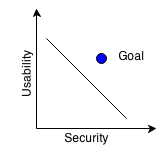
\includegraphics[scale=0.7]{pics/UsabilityVsSecurity.png}
    \end{center}
    \vspace{-20pt}
    \caption{Usability vs. Security}
    \vspace{-10pt}
  \end{wrapfigure}

  Authentication with text-based passwords are a common approach, but it is well known that users often choose weaker passwords because of the limitations of recalling text-based passwords. Graphical passwords came as an alternative solution for overcoming the limitations of text-based passwords, and was inspired by researchers that showed that the graphical memory of humans is particularly well-suited to remember graphical information. The problem with many graphical password schemes is that they often promise improved password memorability and thus usability, while at the same time improving the security \cite{Biddle}. This is why it is important to understand the both usability and security when looking at different password scheme in order to understand the tradeoff between different design choices. 

  {\color{red} \bf Finne forskning som evaluerer grafiske password på usability and memorability}
    
\subsection{Security}

  In knowledge-based authentication, e.g. ``something you know'' we classify attacks into two general categories: guessing and capturing attacks. In a guessing attack the attackers are able to search through the entire password space, or either predict the users passwords patterns in order to avoid searching through the whole passwords space (often referred to as a dictionary attack). This is often associated with the entropy of the password, because the lower the entropy it will be easier to make a successfull attack. When talking about capturing attacks, the attackers are directly obtain the passwords by observing the authentication process. One of the known capturing attacks on graphical passwords are shoulder surfing because of its graphical visualization.  

  Since a person needs to remember a password, it is normally to choose a password that are connected to you as a person in order to remember the password, causing the password to have bias. A bias can be explained as a prejudice in favor of or against one thing, person, or group compared with another, usually in a way that influence a person choice of action. Since psychological studies have recognized that the human brain have a superior memory for recognizing and recalling visual information, it support the statement that users are able to remember more complex graphical password form a larger password space than a alphanumeric password. Logically the attacker then have to build a bigger and more complex dictionary, thus spend more time to achieve the same success rate as for textual passwords. % Her må jeg ha noen eksempler på dictionary attacks mot grafiske passord!!!

  The graphical password scheme DAS \cite{Jermyn} was evaluating the security of their password scheme. They highlighted that there are many factors that impacts the security of a password scheme, like the statement that the users do not use a uniformal distribution of all possible passwords, using Klein's study \cite{UnixPasswords} as a argument. The fact that useres do not pick passwords uniformly is not in itself a sufficient statement to make a guessing attack successful. They try to cover the possibility for a attacker making a successful attack by making their scheme complex, and the results showed that the generated passwords was significantly harder to crack in practice than texutal passwords. The problem is that they used coputer generated passwords that will not show acutally password chosen by user. They did not analyse the security of the DAS including human factors and password biases that may could incluence the practical password space. 

\section{Psychology and passwords}

  \begin{wrapfigure}{r}{0.35\textwidth}
    \vspace{-20pt}
    \begin{center}
      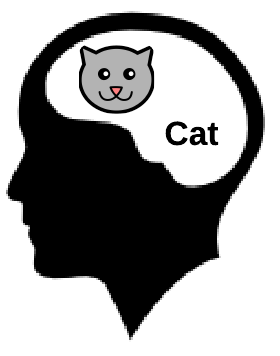
\includegraphics[scale=0.35]{pics/dualCoding.png}
    \end{center}
    \vspace{-20pt}
    \caption{Dual-Coding Theory}
    \vspace{-10pt}
  \end{wrapfigure}

  In many years, the field of psychology been a important in order to understand how humans interpret and remember different information. Psychology studies have recognized that the human brain have a superior memory for recognizing and recalling visual information rather recognizing and recalling verbal or textual information. One known theory is the ``dual-coding theory'', suggesting that verbal and non-verbal memory are processed and represented differently in humans mind. Text are verbal information that is represented symbolically, in contrast to non-verbal information like images that are mentally represented in a way that perceived concepts are assigned to a perceived meaning of what is directly observed. Both verbal and non-verbal information can be used when recalling information. For example, say a person have received stimulus of the concept ``cat'', both the image of a cat as well as the word ``cat''. When the person is asked to recall the concept ``cat'', the person can retrieve the image or the word individually, or both simultaneously. If the word ``cat'' is recalled, the image of the cat is not lost and can still be retrieved at a later point in time. The ability to code a stimulus in two different ways can increase humans ability to remember, in contrast to only code the stimulus in one way. In the background theory there are described three different categories of graphical passwords according to the memory task involved in remembering and entering the password, e.g. recall, recognition and cued-recall. 

  {\bf \color{red} Thorpe and Van Oorschot}
  

\section{Graphical passwords and mobile devices}
  %Intro
  Users are not only dependent on remembering passwords across multiple web pages and systems, but do also need to remember passwords for our small mobile devices. In todays society we're addicted to our mobile devices in our every day life. Mobile devices are not just a communication tool for calling and texting, but also an important tool for every day tasks like doing our work, reading mail, pay our bills and keeping up with our social life. This trend makes our mobile devices vulnerable in terms of security. To avoid unwanted access, smartphones offers different locking mechanisms. The history of locking mechanisms was often a solution solely to prevent accidental use, while current mobile phones require protection in order to secure the potentially vast amount of private data that we keep on our smartphones. Our mobile devices are in rapidly use, leading users to create and reuse shorter passwords and PINs, or no authentication at all. 

  % The time used on unlocking the phone
  In terms of security it is interesting to look at the use of mobile devices and look at the locking habits among users on mobile devices. It is known that services that are rapidly used have weaker password because of the overhead the user needs to spend on typeing their password. In 2014 a group of researchers published a field study of smartphone (un)locking behavior \cite{habits3}. Some of the problems with smartphone users tends to be their rapidly use of their phone. When the device are rabidly use, it results in a lot of time unlocking their phone between every use. In the study they found that there was a significant overhead in the time used of unlocking their phone, where the users participated in the field study used 2.9\% (9\% in the worst case) of their time unlocking their smartphone. 
  
  % The use of locking mechanisms
  Smartphones in use today do not require their users to have a locking mechanism on their smartphone. It is well known that users tends to choose to easiest way out and may result in the choice of not having any locking mechanism at all. Based on the result of the overhead in time used on unlocking their phone, a result may be to take the easiest way out by ignoring the vulnerability of not using a locking mechanism at all. It have been discovered that over 40\% of the users only used a basic ``slide-to-unlock'' mechanism on their smartphone, as well as over 16\% didn't use any locking mechanisms at all \cite{habits3}. This highlights a major bad habit among mobile users. What happens if your mobile is stolen? 

  % Risk vs securtiy
  It is important to understand why people use or not use locking mechanisms on their smartphone. Research have covered that the 46.8\% of the participants agreed or fully agreed that unlocking their phone can be annoying, but at the same time 95.5\% of the somewhat or fully agreed that they liked the idea that their phone was protected \cite{habits3}. This highlights that the users wants to be secure, but there might be a trade-off between the time used to unlock the smartphone vs the security risk.

  One of the popular password schemes on mobile phones are the Android Unlock pattern. It is a graphical password that have been shown to have biases when the password are user-chosen. A research group did a large-scale user study on the Android Unlock Patterns in order to quantify its security \cite{Uellenbeck}. They analyses the biases introduced in the pattern making process and added changes to the scheme in order to avoid the known biases in the password scheme (a description of the Android Unlock Pattern can be found in the background theory). The researchers found that there is a high bias in the pattern selection process, e.g. the upper left corner and three-point long straight lines are very typical selection strategies. If the patterns was uniformly chosen, the probability of starting in the top-left corner should be 11\%, but are instead close to 44\%. Another interesting result is the practical password space used, where about 10\% of all users use less than 190 patterns, while less than 300 patterns capture around 50\% of the whole test population. This shows that a empirical password space are not a representative number when quantifying the security of a password, but we should look at the practical password space, e.g. password that actually are used in practice. The Android Unlock Patterns are a password scheme used on mobile devices. It is important to understand the difference of a password scheme used on a desktop vs. mobile device. As stated earlier a mobile phone have a small screen making it harder to type the password without the standard desktop keyboard. The way that the mobile phone is held, the size of the screen may also impact the way that people write their passwords, but this may need further research to answer. We need to look further into the design space of mobile devices in order to understand how users interact with passwords on mobile devices. 

  